\chapter{Algortimos de Machine Learning}

En este capítulo veremos los principales conocimientos de Aprendizaje automático requeridos para este seminario además se hará énfasis en su clasificación y sus principales algoritmos.

\section*{Aprendizaje Automático}
Machine Learning o aprendizaje automático es una rama de la inteligencia artificial que empezó a cobrar cobrar importancia en los años 80's, en esta rama se diseñan sistemas que aprenden a identificar patrones en un conjunto de datos. A medida que se realice este aprendizaje la máquina podrá ser capaz de realizar una predicción o tomar decisiones sin haber estado programada explícitamente para realizar esta tarea.


El aprendizaje automático se puede clasificar en 3 tipos: Supervizado, No supervisado, Aprendizaje con refuerzo\textbf(cita).
\subsection*{Aprendizaje Supervizado}
Este tipo de aprendizaje toma un conjuto de datos etiquetados como entrada. Primero se entrana el modelo con data de entrada y luego se trata de precedir  una salida. \textquotedblleft El aprendizaje supervisado trata de modelar la relación entre el resultado de la predicción y las características de las entrenadas de manera que se puedan predecir nuevos valores para un nuevo conjunto de datos \textquotedblright \cite{WEBSITE:1}
\subsubsection*{Tipos de problemas}
Dentro del aprendizaje supervisado encontraremos distintos tipos de problemas entre ellos tenemos:
\subsubsection*{Problemas de Regresión Lineal}
Los problemas de regresión lineal son muy conocidos en el ámbito de aprendizaje automático y la estadística 
\subsubsection*{Problemas de Clasificación}
\textquotedblleft En este tipo de problemas se predice una respuesta del tipo categórica de manera que se puedan separar los datos mediante clases. \textquotedblright \cite{WEBSITE:2}

\textquotedblleft El objetivo de los problemas de clasificación es asignar las observaciones en categorías discretas en lugar de estimar valores continuos. \textquotedblright \cite{WEBSITE:1}


\begin{figure}[H]
	\centering
	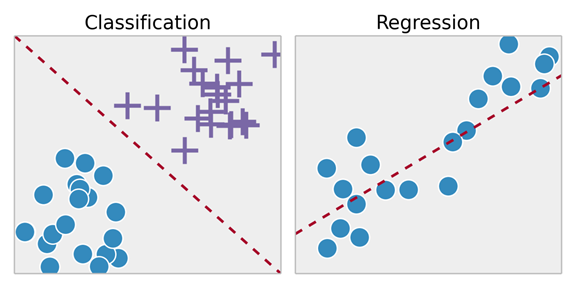
\includegraphics[width=0.9\textwidth]{Figures/regreclas.png}
	\caption{Regresión y clasificación \\ Fuente:  \href{https://medium.com/deep-math-machine-learning-ai/different-types-of-machine-learning-and-their-types-34760b9128a2}{\textit{https://medium.com/}}}
	\label{Regresion}
\end{figure} 

\subsubsection*{Algoritmos de Aprendizaje Supervizado}
\subsubsection*{Regresión Lineal}
\textquotedblleft El modelo de regresión lineal asume que existe una relación entre las variables de entrada $X$ y una salida simple $Y$.  Cuando se tiene solo una variable simple $X$ el método se conoce como simple linear regression y cuando se tienen múltiples entradas se le conoce como multiple linear regression.  \textquotedblright \cite{WEBSITE:3}
\begin{equation}
\label{Simple learning regression}
Y=b_{1}*X+b_{0}
\end{equation} 
Uno de los usos de la regresión lineal es realizar predicciones en un conjunto de datos.
\subsubsection*{Nearest Neighbor}

\subsubsection*{Support Vector Machines (SVM)}
\subsubsection*{Naive Bayes}
\subsubsection*{Decision Trees}
\subsubsection*{Neural Networks}
El tema de Neural Network será tratado con más detenimiento en el capítulo 4.
\subsection*{Aprendizaje No Supervizado}
Mientras que el aprendizaje supervizado aprende  de un conjunto de datos de entrenamiento con respuestas o etiquetas correctas. En el aprendizaje no supervizado los datos de entrenamiento no poseen ninguno tipo de etiqueta, el sistema debe de interpretar los datos por si mismo.
El aprendizaje no supervizado es usado principalmente para el reconocimiento de patrones y modelado descriptivo.
\subsubsection*{Clustering}
Clustering se refiere a agrupar objetos con características similares es decir se busca la relación entre ellos sin necesidad de que exista un conocimiento a priori de esos grupos.
\begin{figure}[H]
	\centering
	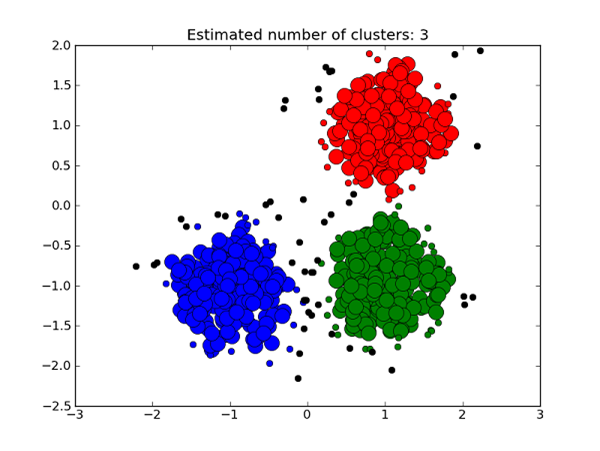
\includegraphics[width=0.9\textwidth]{Figures/clustering.png}
	\caption{Clustering \\ Fuente:  \href{https://medium.com/deep-math-machine-learning-ai/different-types-of-machine-learning-and-their-types-34760b9128a2}{\textit{https://medium.com/}}}
	\label{Clustering}
\end{figure} 
\subsection*{Aprendizaje por refuerzo}
Este tipo de aprendizaje fue inspirado por la psicología conductista, este tipo busca determinar que tipo de acciones tomar en un entorno dado. \textquotedblleft El objetivo del método es recopilar la interacción con el entorno para tomar acciones que maximicen el beneficio o minimicen el riesgo. \textquotedblright \cite{WEBSITE:1}

\section{Deep Learning}

\section{Métodos de optimización}
\section{Redes Neuronales}
\subsection{Neuronas}
En la biología la neurona es conocida como la unidad fundamental del cerebro humano, el cual está compuesto por millones de neuronas interconectadas entre si. El trabajo de las neuronas consiste en recibir información, procesarla y enviarla a otras células. Este modelo fue copiado en 1943 por Warren S. McCulloch y Walter H. Pitts. Analogamente con las neuronas del cerebro humano nuestra neuro artificial toma una cantidad n de entradas $x_{1}, x_{2}, x_{3}, .. , x_{n}$ estas entradas serán multiplicadas por pesos $w_{1}, w_{2}, w_{3}, .. , w_{n}$ además se puede añadir una constante que llamaremos bias. 

La entrada a de la neurona será la suma total de los productos z=  $\sum_{i=1}^{n}x_{i}$ , el valor de z será la entrada a la neurona la cual la evaluará con una función f de tal forma que nuestra salida sea $y=f(z)$. Otra forma de ver esta expresión es por medio de la notación de vectores donde representaremos a las entradas como $x= [x_{1}  x_{2}  x_{3}  ...  x_{n}]$ y los pesos w= $[w_{1}  w_{2}  w_{3}  ...  w_{n}]$ de esta manera la salida de la neurona estará dada por $y=f(x\cdot w+b)$ donde b representa las bias. 

\subsection{Redes Neuronales Artificiales}
Las redes neuronales artificiales(ANN)toman de ejemplo la arquitectura del cerebro como inspiración para la construcción de sistemas inteligente. Actualmente son la base para el desarrollo de la inteligencia artificial. Las redes neuronales están constituidas de las uniones de las neuronas.

\subsection{Redes Neuronales Profundas}


Las redes neuronales profundas estan constituidas principalmente de un numero de capas de convolución, No linearalidad y pooling.
\begin{itemize}
	\item Convolución:
	Un proceso importante dentro de las redes neuronales es la convolución que es usada para detectar las características de una imagen estas características pueden ser bordes, curvas, etc.
	\item No linearalidad:
	Debido a que las convoluciones son operaciones lineales, lo cual no es adecuado para las tareas del mundo real. Debido a esto es importante introducir el ReLu que aplicará funciones no lineales a los mapas de característica producidas en las capas de convolución.
	Una de las funciones las común es ReLu.
	\begin{figure}[H]
		\centering
		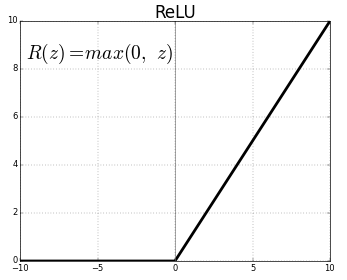
\includegraphics[width=0.5\textwidth]{Figures/relu.png}
		\caption{ReLu}
		\label{ReLu}
	\end{figure}

	
	\item Pooling:
	Sirve para transformar el mapa de características en una representación de menor dimensión con el objetivo de la red sea más invariante a pequeñas transformaciones o variación de la imagen de entrada.
\end{itemize}



%%\subsubsection*{Características}
%%%
%%\begin{figure}[H]
%%\centering
%%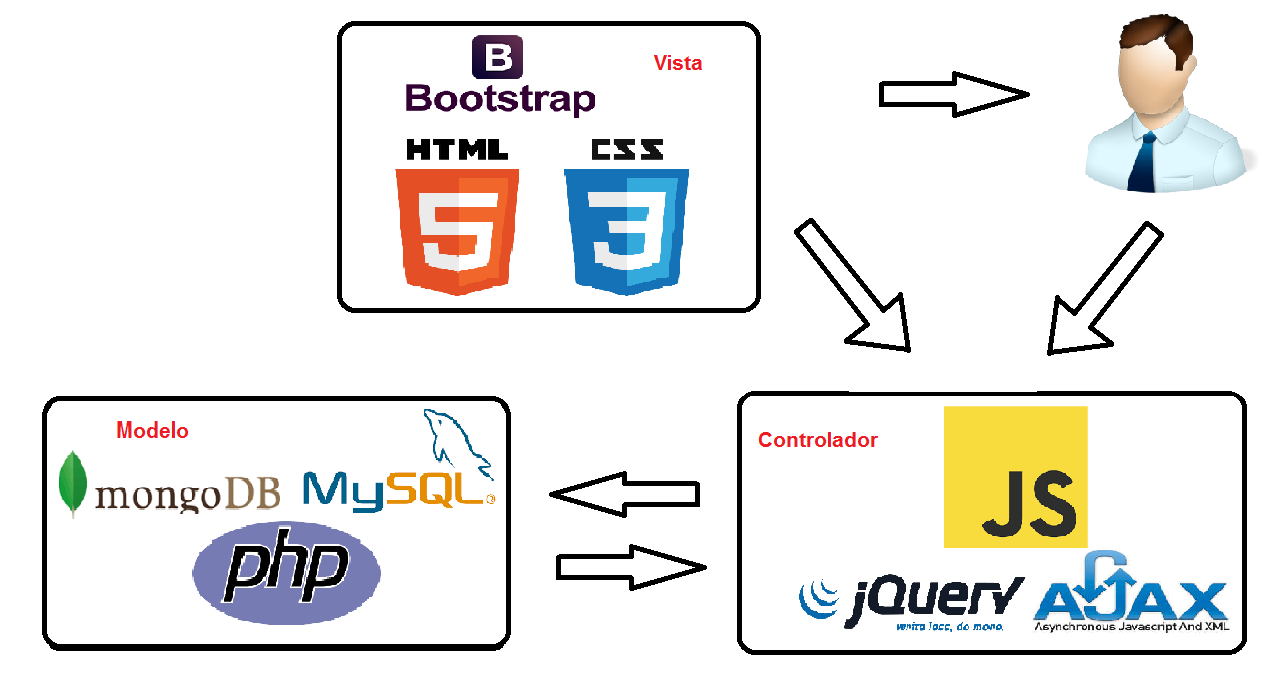
\includegraphics[width=0.9\textwidth]{Figures/mvc.png}
%%\caption{Modelo-Vista-Conrolador}
%%\label{MVC}
%%\end{figure}



\afterpage{\blankpage}